\chapter{解集合プログラミング}\label{chap:asp}

解集合プログラミング(ASP; \cite{%
  Baral03:cambridge,%
  Gelfond88:iclp,%
  Niemela99:amai,%
  Inoue08:jssst})
の言語は,一般拡張選言プログラムをベースとしている.
本稿では説明の簡略化のため,そのサブクラスである
標準論理プログラムについて説明する.
以降,標準論理プログラムを単に論理プログラムと呼ぶ.

\textbf{論理プログラム}は,以下の形式の\textbf{ルール}の有限集合である.
\begin{equation}
  \label{eq:rule}
  a_0\leftarrow a_1,\dots,a_m,\naf{a_{m+1}},\dots,\naf{a_n}
\end{equation}
ここで,
$0\leq m\leq n$ であり,
各$a_i$はアトム,
$\naf{}$は\textbf{デフォルトの否定}
\footnote{\textbf{失敗による否定}とも呼ばれる.述語論理で定義される否定($\neg$)とは意味が異なる.},
``$,$''は連言を表す.
$\leftarrow$の左側を\textbf{ヘッド},右側を\textbf{ボディ}と呼ぶ.
ルールの直観的な意味は,
「$a_1,\ldots,a_m$がすべて成り立ち,$a_{m+1},\ldots,a_n$のそれぞれが成
り立たないならば,$a_0$が成り立つ」である.
ボディが空のルール(すなわち\(a_0\leftarrow\))を\textbf{ファクト}と呼び,
$\leftarrow$を省略してよい.

ヘッドが空のルールを\textbf{一貫性制約}と呼ぶ.
\begin{equation}
  \label{eq:constr}
  \leftarrow a_1,\dots,a_m,\naf{a_{m+1}},\dots,\naf{a_n}
\end{equation}
例えば,一貫性制約
\(\leftarrow a_1,a_2\)は,「$a_1$と$a_2$が両方同時に成り立つことはない」を意味し,
\(\leftarrow a_1, \naf{a_{2}}\)は,「$a_1$が成り立つならば,$a_2$が成り立つ」を意味する.

ASP言語には,組合せ問題を解くために便利な拡張構文が用意されている.
その代表的なものが\textbf{選択子}と\textbf{個数制約}である.
例えば,選択子\(\{a_1;\dots;a_n\}\)をファクトとして書くと,
「アトム集合\(\{a_1,\dots,a_n\}\)の任意の部分集合が成り立つ」を意味する.
個数制約は選択子の両端に選択可能な個数の上下限を付けたものである.
例えば,\(lb\ \{a_1;\dots;a_n\}\ ub \leftarrow Body\)と書くと,
「$Body$が成り立つならば,$a_1,\dots,a_n$のうち,$lb$個以上$ub$個以下
が成り立つ」を意味する.
また,組合せ最適化問題を解くために,最小化関数
(\code{#minimize})・最大化関数(\code{#maximize})等も用意されている.

\textbf{ASPシステム}は,与えられた論理プログラムから,
安定モデル意味論~\cite{Gelfond88:iclp}
に基づく解集合を計算するシステムである.
近年,
{\clingo}~\footnote{\url{https://potassco.org/}},
{\dlv}~\footnote{\url{http://www.dlvsystem.com/dlv/}},
{\wasp}~\footnote{\url{https://www.mat.unical.it/ricca/wasp/}}
など,SATソルバー技術を応用した高速なASPシステムが開発されている.
なかでも{\clingo}は,高性能かつ高機能なASPシステムとして世界中で広く使
われている.

解集合の定義について簡単に説明する.上で述べたように,
論理プログラム$P$は,(\ref{eq:rule})および(\ref{eq:constr})の形
式をしたルール$r$の有限集合である.いくつか表記法を導入する.
\[\head{r}  = a_0 \quad 
  \pbody{r} = \{a_1,\dots,a_m\} \quad
  \nbody{r} = \{a_{m+1},\dots,a_n\}\]
$\head{r}$はルール$r$のヘッドを表す.
ルール$r$が(\ref{eq:constr})の形式の場合,$\head{r}$は空である.
$\pbody{r}$はルール$r$のボディにあるデフォルトの否定が付いていないアト
ムの集合を表す.逆に,
$\nbody{r}$はデフォルトの否定が付いているアトムの集合を表す.
論理プログラム$P$のアトム集合$X$に関する\textbf{リダクト}
$\reduct{P}{X}$を以下のように定義する.
\[\reduct{P}{X}
  =
 \{\head{r}\leftarrow\pbody{r} \mid r\in P, \nbody{r}\cap X=\emptyset\}\]
そして,アトム集合$X$が$\reduct{P}{X}$の最小モデルであるとき,
$X$を$P$の\textbf{解集合}という.

例として,論理プログラム
\(
P = \left\{
    p \leftarrow \naf{q}, \ 
    q \leftarrow \naf{p}
\right\}
\)  
の解集合を考える.以下にアトム集合$X$,リダクト$\reduct{P}{X}$,
$\reduct{P}{X}$の最小モデルを示す.

\[
%\tabcolsep = 2mm
\begin{array}{c|c|c|c}
       X                   & \reduct{P}{X}  & 
\reduct{P}{X}\textrm{の最小モデル}  & X\textrm{は}P\textrm{の解集合?}\\\hline
\{\phantom{p         ,q}\} & \{p\leftarrow,\quad q\leftarrow\}             & \{p,q\}    
&  \times \\\hline
\{         p\phantom{,q}\} & \{p\leftarrow\phantom{\quad q\leftarrow}\}    & \{p\}      
& \circ \\\hline
\{\phantom{p,}        q \} & \{\phantom{p\leftarrow,\quad} q \leftarrow\}  & \{q\}      
& \circ \\\hline
\{         p         ,q \} & \{\phantom{p\leftarrow,\quad q\leftarrow}\}   & \emptyset  
& \times \\\hline
\end{array}
\]

これら4つのアトム集合のうち,
解集合の条件$X=\reduct{P}{X}$を満たすのは,
$\{p\}$と$\{q\}$の2つである.
よって,論理プログラム$P$は$\{p\}$と$\{q\}$の2つの解集合をもつ.

%%%%%%%%%%%%%%%%%%%%%%%%%%%%%%%%%
\begin{table}[tb]
  \centering
  \begin{tabular}{l|*{4}{p{1cm}}}
    論理プログラム &   $\leftarrow$ & $,$        & $;$        & $\sim$       \\\hline
    ソースコード   &   \texttt{:-}  & \texttt{,} & \texttt{;} & \texttt{not}
  \end{tabular}
  \caption{論理プログラムとソースコードの対応}
  \label{tbl:map}
\end{table}
%%%%%%%%%%%%%%%%%%%%%%%%%%%%%%%%%
\begin{figure}[tb]
  \centering
  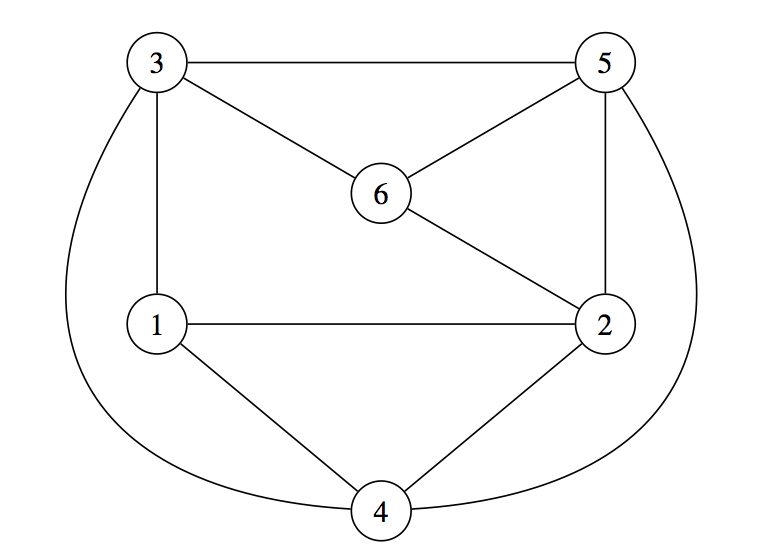
\includegraphics[width=0.6\linewidth]{fig/graph.png}
  \caption{グラフ}
  \label{fig:graph}
\end{figure}
%%%%%%%%%%%%%%%%%%%%%%%%%%%%%%%%%
\lstinputlisting[float=t,caption={%
グラフ彩色問題の論理プログラム (\code{color.lp})},%
captionpos=b,frame=single,label=code:color.lp,%
numbers=left,%
breaklines=true,%
columns=fullflexible,keepspaces=true,%
basicstyle=\ttfamily\scriptsize]{code/color.lp}
%%%%%%%%%%%%%%%%%%%%%%%%%%%%%%%%%
\lstinputlisting[float=t,caption={%
\code{color.lp}に対する{\clingo}の実行例},%
captionpos=b,frame=single,label=code:color.log,%
numbers=none,%
breaklines=true,%
columns=fullflexible,keepspaces=true,%
basicstyle=\ttfamily\scriptsize]{code/color.log}
%%%%%%%%%%%%%%%%%%%%%%%%%%%%%%%%%

解集合プログラミングを用いた問題解法プロセスは,3つのステップからなる.
まず最初に,解きたい問題を論理プログラムとして表現する.
つぎに,ASP システムを用いて,論理プログラムの解集合を計算する.
最後に,解集合を解釈して元の問題の解を得る.
%
ここでは,グラフ彩色問題を例として,各ステップ毎に解法プロセスを説明する.
ASP システムとしては{\clingo}を用いる.
以降で示す論理プログラムのソースコードはすべて{\gringo}言語で書かれて
おり,表記上の対応については表~\ref{tbl:map}の通りである.

グラフ彩色問題とは,辺で結ばれたノードが同じ色にならないように,各ノー
ドを塗り分ける問題である.
例として,図~\ref{fig:graph}のグラフを赤(\code{r}),青(\code{b}),緑
(\code{g})の3色で塗り分ける問題を考える.
この問題を表す論理プログラムをコード~\ref{code:color.lp}に示す.

2〜4行目は,ノード(\code{node})と辺(\code{edge})をファクトとし
て書くことによって,図~\ref{fig:graph}のグラフを表している.
ピリオド(``\code{.}'')はルールの終わりを表す終端記号である.
7行目も同じく,色(\code{col})をファクトで表している.
%
10行目のルールは,個数制約を使って「各ノードは一つの色で塗られる」とい
う制約を表している.アトム\code{color(X,C)}は,ノード\code{X}が色
\code{C}で塗られることを意味する.セミコロン(\code{:})は条件付きリテラ
ルと呼ばれる拡張構文であり,このルールのヘッドは,
\code{1 \{ color(X,r);color(X,b);color(X,g) \} 1}のように展開される.
11行目のルールは,一貫性制約を使って「辺で結ばれたノード(\code{X}と
\code{Y})は,同じ色(\code{C})で塗られない」という制約を表している.

ASP システムは解集合を計算して出力する.
コード~\ref{code:color.log}に{\clingo}の実行例を示す.
この出力から,ノード1と5は緑,ノード4と6は赤,ノード2と3は青に塗り分け
られることがわかる.

%%% Local Variables:
%%% mode: japanese-latex
%%% TeX-master: "paper"
%%% End:
